%%%%%%%%%%%%%%%%%%%%%%%%%%%%%%%%%%%%%%%%%%%%%%
% Descripción completa del vehículo
%%%%%%%%%%%%%%%%%%%%%%%%%%%%%%%%%%%%%%%%%%%%%%
\chapter{Componentes del vehículo}
Las características técnicas del vehículo a nivel constructivo se pueden encontrar en la página web del fabricante \cite{Greenland} (\textit{Changzhou Greenland Vehicle Co., Ltd,}) y se muestran en la tabla \ref{Tab:medidas_UALeCARM} para facilitar la labor.

\begin{table}[H]
\caption{Características técnicas del vehículo \textit{UAL-eCARM}.}\label{Tab:medidas_UALeCARM}
\centering
\begin{tabular}{|c |c |c |c|}
\hline % inserts single horizontal line
Parámetro & Medida & Parámetro & Medida \\
\hline
Longitud & 2680 mm  &  Velocidad máxima &  45km/h  \\
\hline
Anchura &  1510 mm  & Autonomía & 90 km \\
\hline
Altura & 1780 mm  & Radio de giro mínimo & 4.3 m \\
\hline
Distancia entre ejes &  1830 mm  & Peso & 740 kg \\
\hline
Paso ruedas traseras & 1285 mm  & Peso sin baterías &  460 kg \\
\hline
Paso ruedas delanteras & 1260 mm  &  Peso máximo &  950 kg \\
\hline
Pendiente máxima &  20\% &  Potencia máxima & 4.3 kW \\
\hline
\end{tabular}
\end{table}

\section{Energía}
La fuente de energía que posee el vehículo son 8 baterías de gel electrolítico de ácido-plomo reguladas por válvula (VRLA) marca Trojan, Figura \ref{fig:Bateria}. Anteriormente se disponía de 8 baterías de la marca \textit{Greensaver} modelo \textit{SP210-6}, Figura \ref{fig:Bateria-ant}. Para acceder a ellas se debe levantar la parte inferior de los asientos del vehículo, Figura \ref{fig:baterias-asientos}. Estas baterías suministran una tensión de 6 Voltios (V) y poseen una capacidad de 189 Amperio-hora (Ah). Con estas características, su conexión se produce en serie obteniendo una tensión total para distribuir en el vehículo de 48V. A pesar de que la tensión suministrada es de 48V, se considera necesario el empleo de conversores DC-DC que suministren líneas de tensión a 5V, 12V y 24V, puesto que no todos los dispositivos electrónicos que incorpora el vehículo trabajan a igual tensión.

\begin{figure}[!ht]
\begin{center}
	\subfloat[Trojan 6V-GEL.]{
		\label{fig:Bateria}
		\includegraphics[width=0.35\textwidth]{Figuras/C3-Bateria}}
	\subfloat[Greensaver SP210-6.]{
		\label{fig:Bateria-ant}
		\includegraphics[width=0.4\textwidth]{Figuras/C3-Bateria-ant}}
	\caption{Baterías instaladas en el vehículo.}
\end{center}
\end{figure}

\begin{figure}[!ht]
  \centering
    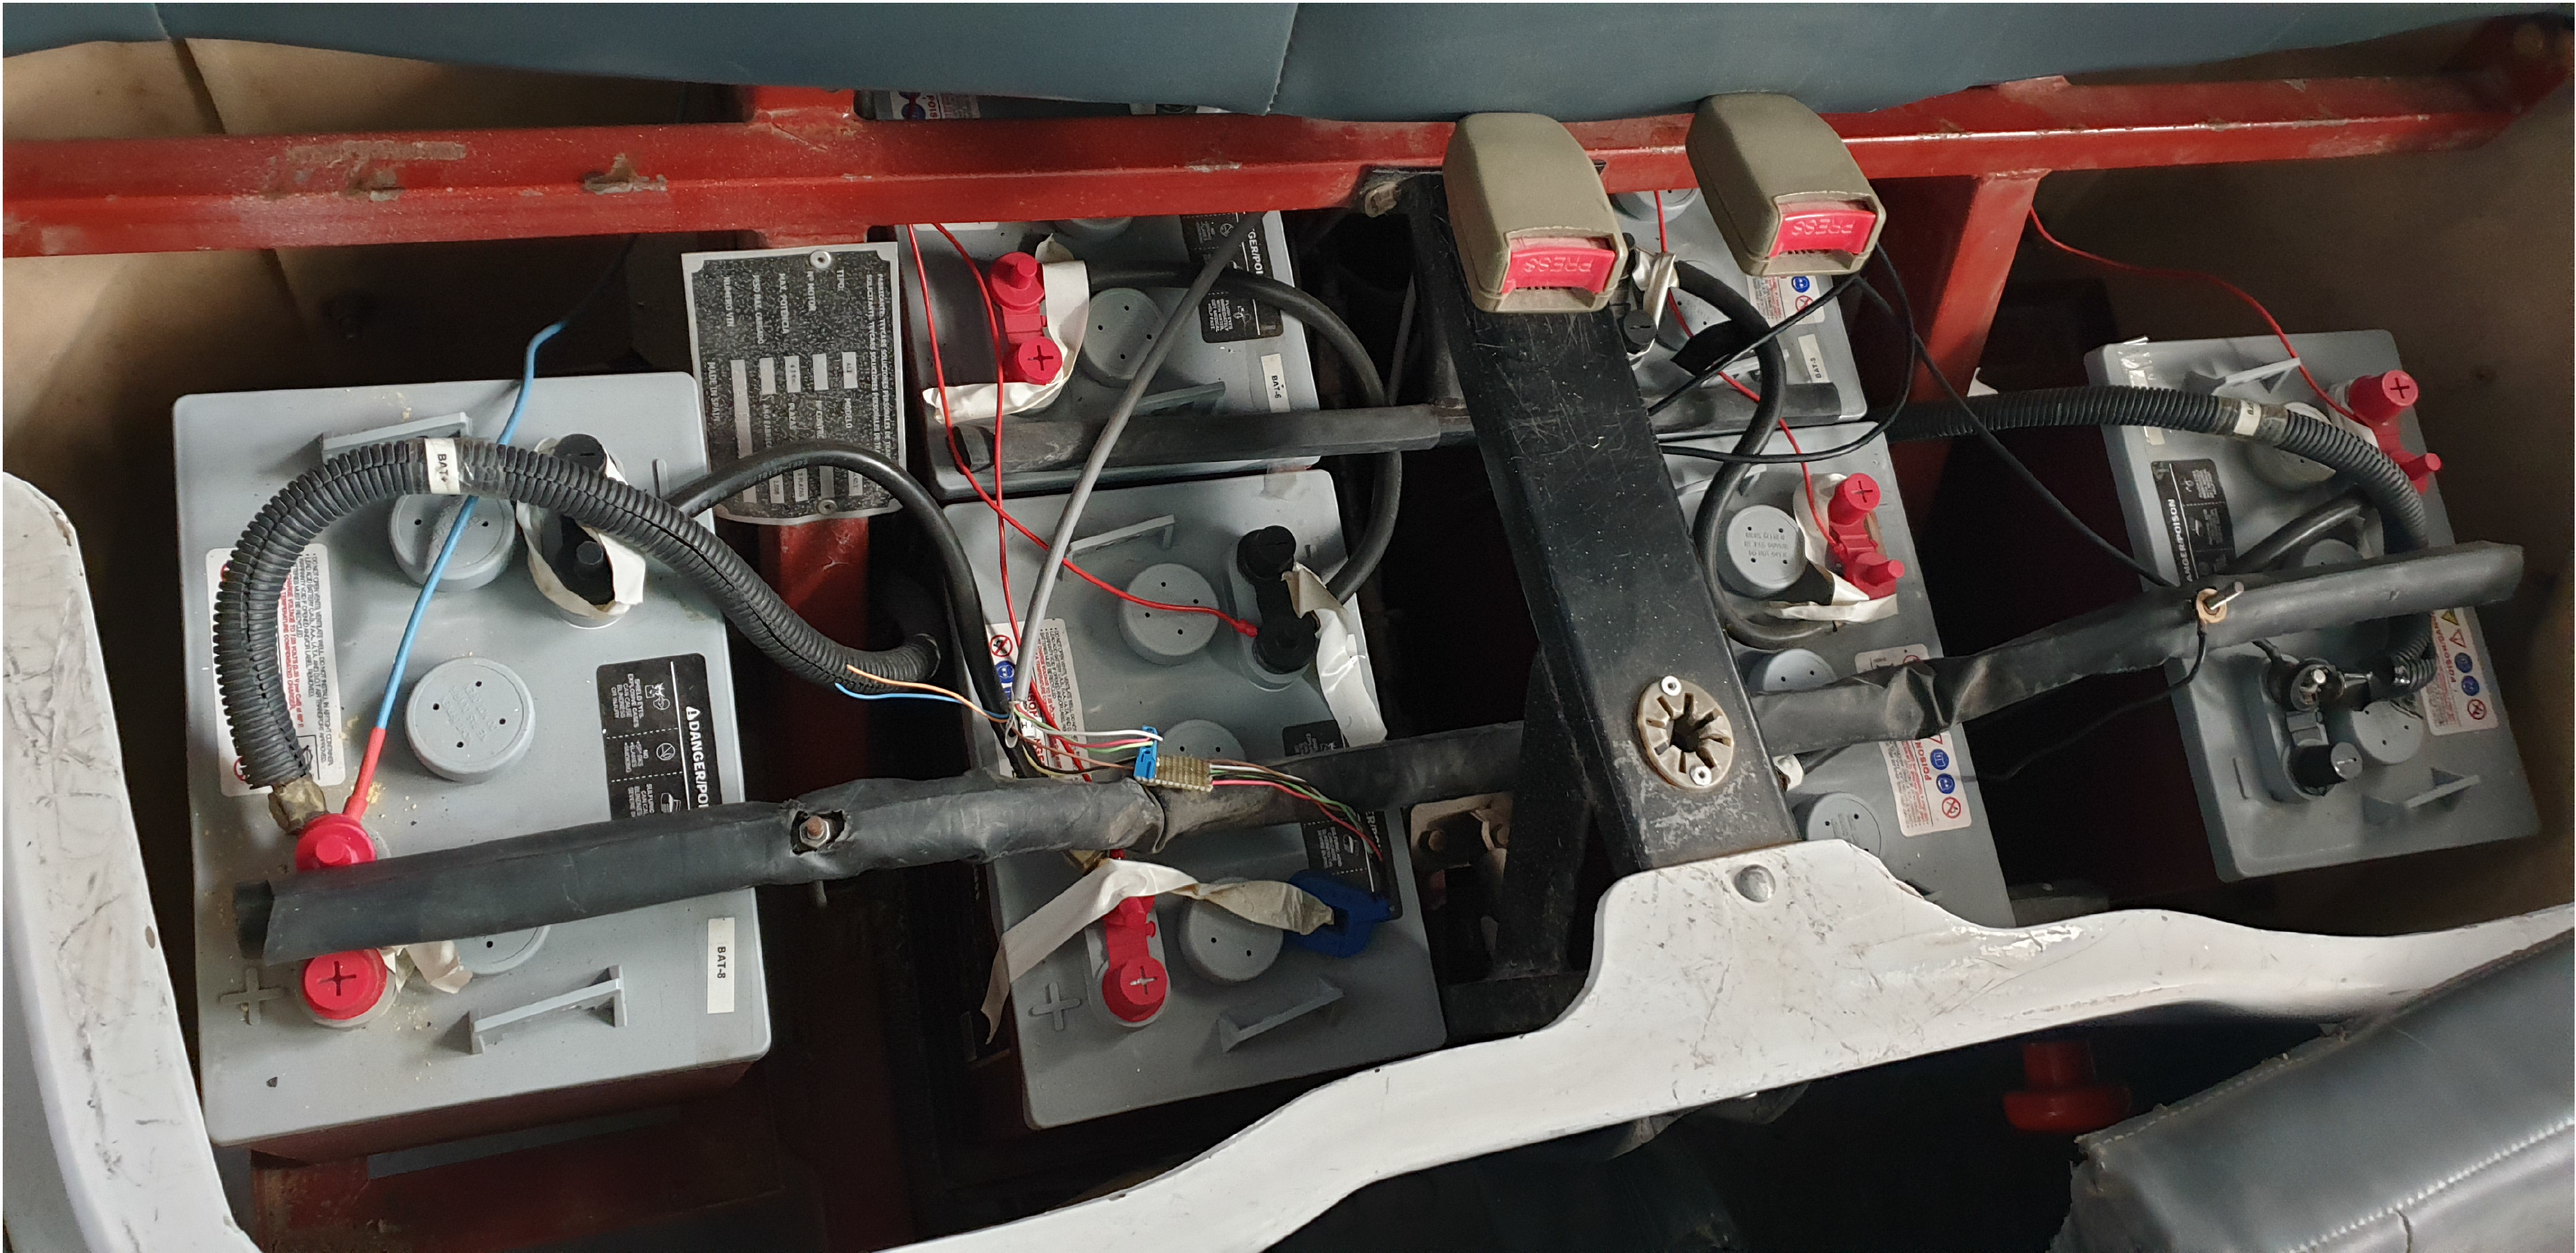
\includegraphics[width=1\textwidth]{Figuras/C3-Baterias-instalacion}
  \caption{Ubicación de las baterías en el vehículo.}
  \label{fig:baterias-asientos}
\end{figure}

\subsection{PowerBox}
Este componente, Figura \ref{fig:PowerBox}, presenta tres funciones principales:
\begin{itemize}
\item Proteger la instalación electrónica mediante la instalación previa de un fusible de 20A.

\item Encender los distintos componentes de forma individual o en pequeñas agrupaciones que permite evitar consumo innecesario de componentes que no se usan.

\item Cortar la alimentación de distintos elementos para manipularlos sin tener que apagar el vehículo entero.
\end{itemize}

A esta caja están conectadas las dos fuentes CC-CC, los dos reguladores y el PC industrial. Como protección principal se emplea un fusible de 20A a la entrada y un display que monitoriza la tensión, intensidad y consumo de todos los componentes conectados. Además se han implementado cinco interruptores que modularizan el encendido de cada componente y uno de ellos actúa como interruptor principal. Esto permite cierto nivel de ahorro energético que se produciría por el encendido de componentes que no se empleen en dicho momento y el encendido de componentes de forma individual para realizar ensayos sobre ellos.  

\subsection{Fuentes de alimentación}
Las baterías, como ya se comentó en la introducción de esta sección, suministran una tensión de 48V, pero no todos los dispositivos requieren dicha tensión. Para el establecimiento de las distintas tensiones requeridas se han empleado dos fuentes CC-CC las cuales convierten de 48V a 12V y 24V respectivamente y dos reguladores conmutados de 5V y 19V respectivamente. 

La fuente CC-CC de 24V, SD-500L-24 mean well (ver figura \ref{fig:FuenteDC}), se emplea para la alimentación del motor de la dirección, de los distintos amperímetros de la marca LEM situados por el vehículo (Baterías y motor) y el sensor láser de la parte frontal. La fuente de 12V, reutilizada de otros proyectos realizados anteriormente, suministra corriente al amperímetro Honeywell que cuantifica la corriente suministrada por las baterías. El regulador de 5V localizado en la caja denominada \textit{PowerBox} se emplea para la alimentación de aquella electrónica que opera a dicho nivel. El regulador de 19V se requiere para el funcionamiento del monitor situado en la cabina del vehículo. Para su correcto funcionamiento, puesto que el dispositivo integrado abarca un rango de tensiones de salida de 11.85V-22V, se construye un circuito físico para adecuar la tensión a 19V, figura \ref{fig:Regulador}.

\begin{figure}[h!]
\begin{center}
	\subfloat[Fuente CC-CC.]{
		\label{fig:FuenteDC}
		\includegraphics[width=0.3\textwidth]{Figuras/C3-DCDC}}
	\subfloat[Regulador.]{
		\label{fig:Regulador}
		\includegraphics[width=0.3\textwidth]{Figuras/C3-Regulador}}
	\subfloat[PowerBox.]{
		\label{fig:PowerBox}
		\includegraphics[width=0.35\textwidth]{Figuras/C3-PowerBox}}
	\caption{Componentes encargados de la administración de corriente.}
\end{center}
\end{figure}

\textbf{HAY QUE AÑADIR UN ESQUEMA QUE MUESTRE EL CABLEADO ELÉCTRICO DE LA ALIMENTACIÓN DEL VEHÍCULO}

\section{Tracción}

\section{Dirección}

\section{Otros sensores}


Describir TODO lo que hay instalado en el vehículo. Descripción completa y muy detallada de todos los componentes, características, hojas de fabricantes, que variables generan, si están estandarizadas o no, como se comunican con ROS, ... Incluir comentarios en cursiva con las apreciaciones de los que estén trabajando con ellos, como pequeños trucos o imperfecciones que haya que considerar y aún no se sepa porqué aparecen.

\section{Tareas Pendientes}
Cosas a instalar o calibrar.